
\documentclass[11pt,a4paper]{article}
\usepackage[utf8]{inputenc}
\usepackage[T1]{fontenc}
\usepackage{lmodern}
\usepackage[margin=2.2cm]{geometry}
\usepackage{microtype}
\usepackage{graphicx}
\usepackage{booktabs}
\usepackage{longtable}
\usepackage{tabularx}
\usepackage{array}
\usepackage{float}
\usepackage{fancyhdr}
\usepackage{xcolor}
\usepackage{hyperref}
\usepackage{enumitem}
\usepackage{setspace}
\usepackage{caption}
\usepackage{titlesec}
\usepackage{amsmath}
\usepackage{pdflscape}
\usepackage{verbatim}
\definecolor{accent}{HTML}{1F4E79}
\definecolor{soft}{HTML}{EAF1F7}
\definecolor{textgray}{HTML}{4D5966}
\hypersetup{colorlinks=true, linkcolor=accent, citecolor=accent, urlcolor=accent, pdftitle={MAS LCE project compendium}}
\pagestyle{fancy}
\fancyhf{}
\fancyfoot[C]{\thepage}
\renewcommand{\headrulewidth}{0pt}
\setstretch{1.06}
\titleformat{\section}{\Large\bfseries\color{accent}}{\thesection}{0.6em}{}
\titleformat{\subsection}{\large\bfseries\color{accent}}{\thesubsection}{0.6em}{}
\captionsetup{font=small,labelfont=bf}
\setlength{\parskip}{0.5em}
\setlength{\parindent}{0pt}

\begin{document}

{\color{accent}\rule{\textwidth}{1.2pt}}
\begin{center}
    {\LARGE\bfseries Toward an Actionable Model for Proactive Detection of Fraudulent Online Classified Ads}\\[0.4em]
    {\large David Graz and OpenAI}\\[0.8em]
    {\small March 2026}
\end{center}
{\color{accent}\rule{\textwidth}{0.6pt}}

\section*{Abstract}
This article reconstructs and redesigns, in English and in article form, the 2024 MAS LCE master thesis by David Graz on the proactive detection of fraudulent online classified ads. The reconstructed study asks a practical operational question: how can suspicious listings be detected efficiently and reliably before they generate additional victims? The archived project combines a ratified research design, a completed thesis, defense slides, interview material, quantitative data files, scripts, and supporting literature. The underlying model operationalises three indicators---price anomaly, content similarity or duplication, and profile recency---within an actionable fraud index inspired by the actionable-knowledge framework of Avenier and Schmitt, Ribaux's indicia methodology, and Dupont's ecosystemic view of cybercrime. Reproduction required canonicalisation because multiple file versions coexist in the archive. Using the canonical exploratory sample ($n=315$) and the canonical case-study sample ($n=2166$), the compendium reproduces the thesis' descriptive counts and closely reproduces its predictive metrics. The case-study random-forest model reaches accuracy 0.954, precision 0.940, recall 0.975, specificity 0.930, and AUC 0.978. The study's main contribution is therefore best understood as an operational triage model for index-based fraud risk, not as a final adjudicative classifier of legally proven fraud. Within that scope, the reconstructed research remains coherent and practically relevant.

\textbf{Keywords:} online classified ads; fraud detection; money mules; actionable knowledge; cybercrime; fraud risk indexing

{\newpage}

\section{Introduction}
Fraudulent classified ads sit at the intersection of cyber-enabled fraud, digital consumer risk, and intelligence-led policing. In the original Graz study, the problem was framed around low-value but high-volume online fraud capable of recruiting money mules, facilitating phishing-like payment diversion, and eroding trust in e-commerce. The core question was operational rather than purely theoretical: how can fraudulent online listings be detected \emph{efficiently} and \emph{reliably}? The project proposed that three recurring signs---an implausibly low asking price, repeated or duplicated content, and recently created or opaque seller profiles---could be translated into an actionable model for proactive detection.

That proposition is consistent with three strands of literature. First, Avenier and Schmitt argue that research for action should transform dispersed practitioner know-how into knowledge that can guide decisions and intervention \cite{avenier2007}. Second, Ribaux treats traces and indicia as operational elements of investigation rather than passive remnants \cite{ribaux2023}. Third, Dupont's ecosystemic account of cybercrime highlights that online security is distributed across platforms, law enforcement, intermediaries, and users rather than monopolised by a single actor \cite{dupont2024}. The literature on classified-ad fraud and related scam ecosystems likewise points to unusually attractive offers, repeated content, weak profile credibility, and evasive payment practices as persistent red flags \cite{alrousan2020, alzghoul2024, jacquart2021, mokhberi2024}.

The purpose of the present reconstruction is twofold. First, it redesigns the original thesis as a concise article in English. Second, it anchors the study inside a reproducible research compendium that makes the quantitative evidence and its limitations explicit. The companion audit report documents the full integrity review; the present article focuses on the research argument and on the substantive findings that remain robust after canonicalisation.

\section{Theoretical framing and model logic}
The study's conceptual move is to reframe fraud detection as an actionable-knowledge problem. Rather than searching for a universal and static fraud signature, the project organises practitioner observations into a small set of operational indicators that can be scored, communicated, and revised. The three indicators are straightforward:
\begin{enumerate}[leftmargin=1.4em]
    \item \textbf{Price anomaly}: the lower the price relative to a market benchmark, the stronger the suspicion that the offer is strategically attractive rather than economically grounded.
    \item \textbf{Content similarity or duplication}: repeated textual patterns suggest mass publication, template reuse, or automated listing behaviour.
    \item \textbf{Profile recency or opacity}: missing or recently created profiles are interpreted as more suspicious than older, stable profiles.
\end{enumerate}

The original project translated these indicators into a fraud index and then into a binary operational target: \emph{acceptable} versus \emph{unfavorable} fraud risk. This is a key point for interpretation. The study does not claim that every unfavorable listing is proven fraud. Instead, it proposes an \emph{index-based probability of fraud} that can support triage, warning, and preventive intervention.

\begin{figure}[H]
    \centering
    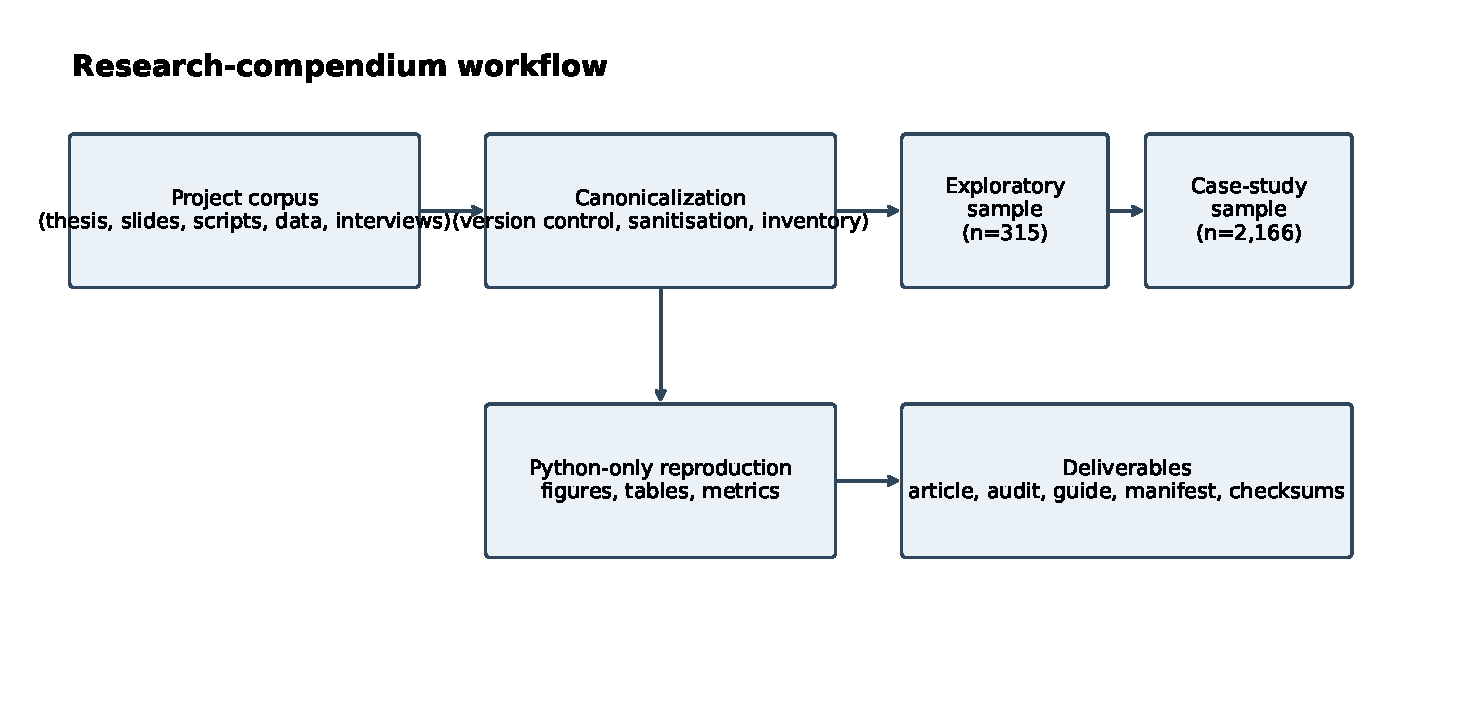
\includegraphics[width=0.95\textwidth]{../figures/workflow_overview.pdf}
    \caption{Workflow used in the final research compendium: source corpus, canonicalisation, quantitative reproduction, and final deliverables.}
\end{figure}

\section{Materials and methods}
\subsection{Source corpus and reconstruction strategy}
The archived MAS LCE corpus is unusually rich for a master-level project. The compendium inventoried 1024 files across scripts, interview materials, theory notes, quantitative data, diagrams, and literature. Not all bundled files were analytically equivalent: some were earlier drafts, some were later refinements, and some were obsolete or unsafe to reuse. Reconstruction therefore proceeded by identifying canonical files, sanitising sensitive material, and preserving a full source inventory.

\subsection{Qualitative phase}
The qualitative phase rests on six exploratory interviews with nine cybercrime practitioners from several francophone Swiss cantons. The original project used thematic analysis to convert practitioner observations into operational categories. Across the archived interview reports and thematic-analysis note, seven themes recur: fragmented responsibilities, recurring fraud indicators, the absence of proactive tools, the international dimension of the phenomenon, prevention as leverage, pessimism about trend evolution, and bottlenecks in cooperation.

\subsection{Quantitative phase}
Two canonical datasets were identified in the archive. The exploratory verification sample contains 315 listings and focuses on suspicious iPhone listings gathered to test the theoretical model. The broader case-study sample contains 2166 listings and serves as the main quantitative stress test. Table~\ref{tab:data-sources} summarises the reconstructed data basis.

\begin{table}[H]
\centering
\caption{Canonical quantitative basis used in the reconstruction.}
\label{tab:data-sources}
\begin{tabularx}{0.78\textwidth}{p{6.2cm} X}
\toprule
Item & Value \\
\midrule
Exploratory sample size & 315 \\
Exploratory acceptable risk & 34 \\
Exploratory unfavorable risk & 281 \\
Case-study sample size & 2166 \\
Case-study acceptable risk & 1015 \\
Case-study unfavorable risk & 1151 \\
\bottomrule
\end{tabularx}
\end{table}

The operational structure follows the original thesis. Price anomaly is scored against model-specific benchmark prices. Text similarity is represented through archived content scores derived from duplication logic. Profile recency is captured by the year of profile creation or by missingness when the platform exposed no usable profile age. These indicator scores are summed into a fraud index, which is then thresholded into acceptable versus unfavorable risk. The predictive stage uses a random-forest classifier with cross-validation to reproduce the archived model family.

\section{Results}
\subsection{Descriptive reconstruction}
The canonical exploratory sample reproduces the thesis' core descriptive totals: 114 detected listings, 80 identified listings, 7 manually negative listings, and 114 positive listings, alongside 34 acceptable-risk and 281 unfavorable-risk cases. The canonical case-study sample reproduces the broader stress-test totals: 1,546 detected listings, 259 identified listings, 343 negative listings, and 18 positive listings, alongside 1,015 acceptable-risk and 1,151 unfavorable-risk cases.

The qualitative and descriptive layers point in the same direction. Price anomalies cluster strongly in the unfavorable-risk group. Content duplication is common among suspicious listings. Older profiles are disproportionately associated with acceptable-risk cases, whereas newly created or intermediate profiles dominate the unfavorable-risk group. The case-study classifier reproduces the strongest and most publication-ready quantitative result in the thesis: high discrimination between acceptable and unfavorable risk categories.

\begin{figure}[H]
    \centering
    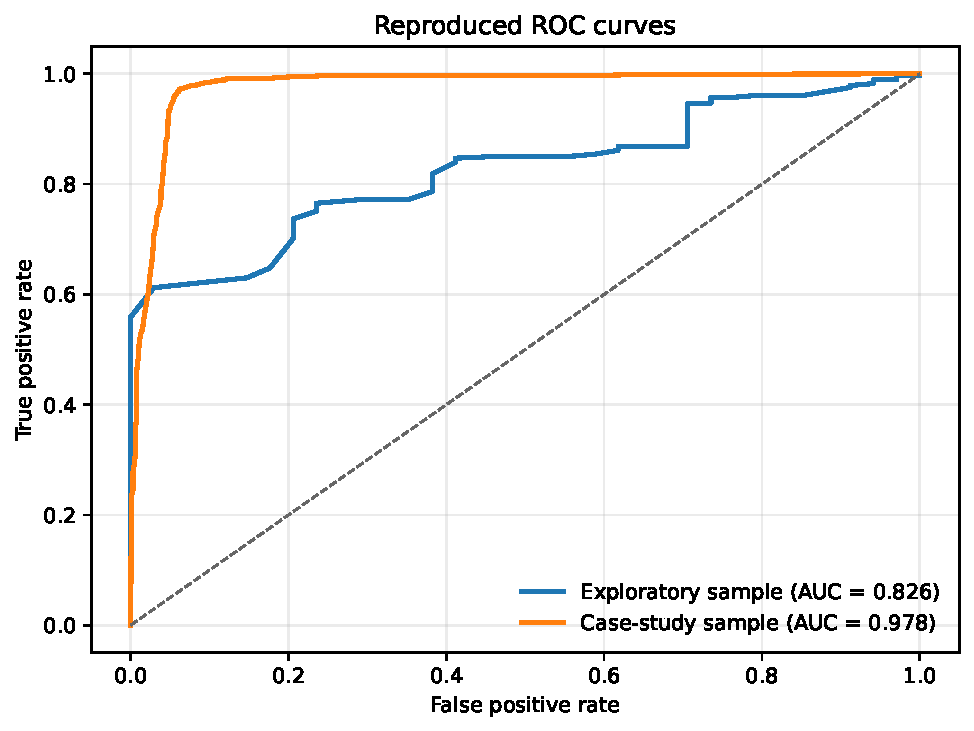
\includegraphics[width=0.80\textwidth]{../figures/roc_curves.pdf}
    \caption{Cross-validated ROC curves reproduced from the canonical exploratory and case-study datasets.}
\end{figure}

\begin{figure}[H]
    \centering
    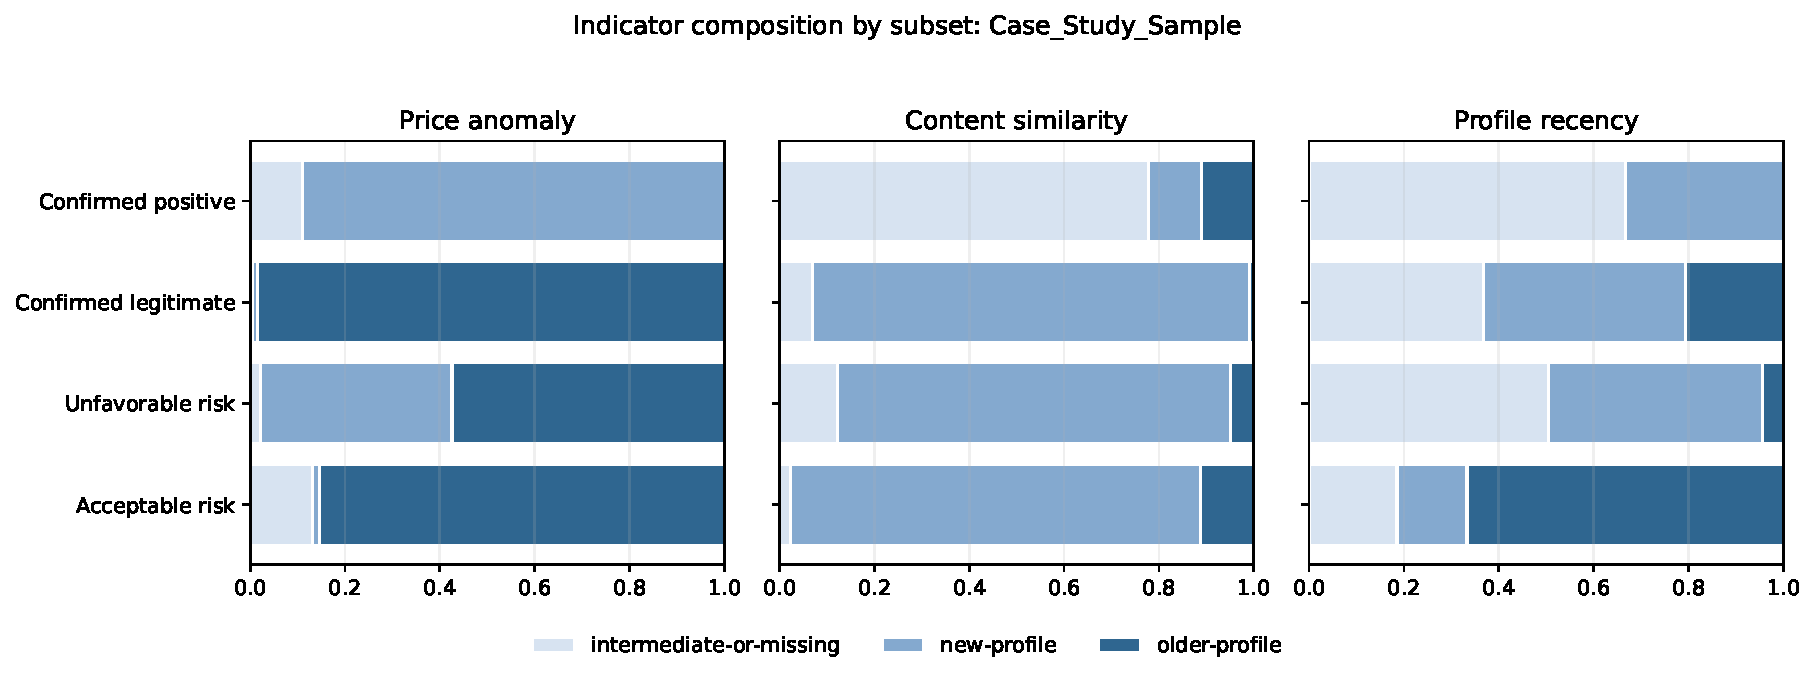
\includegraphics[width=0.98\textwidth]{../figures/case_indicator_distribution.pdf}
    \caption{Indicator composition in the canonical case-study dataset. The confirmed-positive row uses the archive's manually confirmed positive cases only.}
\end{figure}

\begin{table}[H]
\centering
\caption{Reproduced predictive performance.}
\begin{tabularx}{\textwidth}{p{4.6cm} c c c c c c}
\toprule
Evaluation & Accuracy & Precision & Recall & F1 & Specificity & AUC \\
\midrule
Exploratory sample (original script) & 0.873 & 0.914 & 0.947 & 0.930 & 0.265 & 0.826 \\
Exploratory sample (clean rerun) & 0.879 & 0.912 & 0.957 & 0.934 & 0.235 & 0.841 \\
Case-study sample (canonical script) & 0.954 & 0.940 & 0.975 & 0.957 & 0.930 & 0.978 \\
\bottomrule
\end{tabularx}
\end{table}

\section{Discussion}
Three points emerge from the reconstruction. First, the project's real innovation is not a novel machine-learning architecture; it is the operational formalisation of practitioner knowledge into a compact fraud index. That is what makes the model actionable. Second, the results support an ecosystemic interpretation of fraud prevention. Because responsibilities are distributed across platforms, police services, and users, the model is most valuable as a shared triage language rather than as a stand-alone enforcement tool. Third, the strongest quantitative results concern consistency with an internal risk target. This is still useful: a platform-side warning system or analyst triage queue often needs a calibrated suspicion index before it needs courtroom-grade proof.

The reconstructed study therefore converges on a practical message already visible in the interviews: low prices, repeated language, and weak profile credibility are jointly useful for proactive screening. At the same time, the model should be interpreted as a preventive-risk device, not as a substitute for case-by-case investigation.

\section{Limitations}
The reconstructed study remains bounded by the original design. The datasets are platform-specific and product-heavy, with iPhone listings playing a central role. The target variable is index-based, not a comprehensive archive of adjudicated fraud outcomes. Ground truth is strongest at the extremes---confirmed positives and confirmed negatives---and weakest in the large middle of detected or identified but not fully adjudicated listings. Finally, the project archive contains multiple data versions, which means that quantitative reproduction depends on selecting canonical files rather than treating every bundled copy as equivalent.

\section{Conclusion}
Reconstructed as an article and backed by a documented Python compendium, the Graz MAS LCE project offers a credible and practically relevant approach to proactive detection of fraudulent online classified ads. The evidence supports the usefulness of a three-indicator operational model built around price anomaly, content reuse, and profile recency. The broader lesson is methodological: in fast-moving cybercrime settings, operational value often comes from converting scattered practitioner knowledge into transparent, auditable, and updateable indices. Read in that way, the project succeeds. It provides a defensible starting point for a pilot deployment, while the companion integrity audit clarifies the data-governance and evaluation work still needed for stronger publication-grade claims.

{\newpage}

\begin{thebibliography}{99}
\bibitem{alrousan2020} Al-Rousan, S., Abuhussein, A., Alsubaei, F., Collen, L., \& Shiva, S. (2020). Ads-Guard: Detecting scammers in online classified ads. \emph{2020 IEEE Symposium Series on Computational Intelligence}, 1492--1498.
\bibitem{alzghoul2024} Alzghoul, J. R., Abdallah, E. E., \& Al-khawaldeh, A. S. (2024). Fraud in online classified ads: Strategies, risks, and detection methods. \emph{Journal of Applied Security Research, 19}(1), 45--69.
\bibitem{avenier2007} Avenier, M.-J., \& Schmitt, C. (2007). \emph{La construction de savoirs pour l'action}. Paris: L'Harmattan.
\bibitem{dupont2024} Dupont, B. (2024). \emph{La cybercriminalité: Approche écosystémique de l'espace numérique}. Paris: Armand Colin.
\bibitem{jacquart2021} Jacquart, B., Schopfer, A., \& Rossy, Q. (2021). Mules financières: profils, recrutement et rôles de facilitateur pour les escroqueries aux fausses annonces. \emph{Revue internationale de criminologie et de police technique et scientifique, 74}(4), 409--426.
\bibitem{mokhberi2024} Mokhberi, A., Huang, Y., Humbert, G., Obada-Obieh, B., Mehrabi Koushki, M., \& Beznosov, K. (2024). Trust, privacy, and safety factors associated with decision making in P2P markets based on social networks. \emph{Proceedings of the 2024 CHI Conference on Human Factors in Computing Systems}, 1--25.
\bibitem{ribaux2023} Ribaux, O. (2023). \emph{De la police scientifique à la traçologie: Le renseignement par la trace}. Lausanne: PPUR.
\bibitem{rossy2020} Rossy, Q., \& Borisova, B. (2020). Escroqueries par Internet. In \emph{Cybercrimes et enjeux technologiques: Contexte et perspectives} (pp. 227--250).
\bibitem{saumya2022} Saumya, S., \& Singh, J. P. (2022). Spam review detection using LSTM autoencoder: An unsupervised approach. \emph{Electronic Commerce Research, 22}(1), 113--133.
\end{thebibliography}

\end{document}
